
%% bare_conf.tex
%% V1.4b
%% 2015/08/26
%% by Michael Shell
%% See:
%% http://www.michaelshell.org/
%% for current contact information.
%%
%% This is a skeleton file demonstrating the use of IEEEtran.cls
%% (requires IEEEtran.cls version 1.8b or later) with an IEEE
%% conference paper.
%%
%% Support sites:
%% http://www.michaelshell.org/tex/ieeetran/
%% http://www.ctan.org/pkg/ieeetran
%% and
%% http://www.ieee.org/

%%*************************************************************************
%% Legal Notice:
%% This code is offered as-is without any warranty either expressed or
%% implied; without even the implied warranty of MERCHANTABILITY or
%% FITNESS FOR A PARTICULAR PURPOSE! 
%% User assumes all risk.
%% In no event shall the IEEE or any contributor to this code be liable for
%% any damages or losses, including, but not limited to, incidental,
%% consequential, or any other damages, resulting from the use or misuse
%% of any information contained here.
%%
%% All comments are the opinions of their respective authors and are not
%% necessarily endorsed by the IEEE.
%%
%% This work is distributed under the LaTeX Project Public License (LPPL)
%% ( http://www.latex-project.org/ ) version 1.3, and may be freely used,
%% distributed and modified. A copy of the LPPL, version 1.3, is included
%% in the base LaTeX documentation of all distributions of LaTeX released
%% 2003/12/01 or later.
%% Retain all contribution notices and credits.
%% ** Modified files should be clearly indicated as such, including  **
%% ** renaming them and changing author support contact information. **
%%*************************************************************************


% *** Authors should verify (and, if needed, correct) their LaTeX system  ***
% *** with the testflow diagnostic prior to trusting their LaTeX platform ***
% *** with production work. The IEEE's font choices and paper sizes can   ***
% *** trigger bugs that do not appear when using other class files.       ***                          ***
% The testflow support page is at:
% http://www.michaelshell.org/tex/testflow/



\documentclass[conference]{IEEEtran}
% Some Computer Society conferences also require the compsoc mode option,
% but others use the standard conference format.
%
% If IEEEtran.cls has not been installed into the LaTeX system files,
% manually specify the path to it like:
% \documentclass[conference]{../sty/IEEEtran}





% Some very useful LaTeX packages include:
% (uncomment the ones you want to load)


% *** MISC UTILITY PACKAGES ***
%
%\usepackage{ifpdf}
% Heiko Oberdiek's ifpdf.sty is very useful if you need conditional
% compilation based on whether the output is pdf or dvi.
% usage:
% \ifpdf
%   % pdf code
% \else
%   % dvi code
% \fi
% The latest version of ifpdf.sty can be obtained from:
% http://www.ctan.org/pkg/ifpdf
% Also, note that IEEEtran.cls V1.7 and later provides a builtin
% \ifCLASSINFOpdf conditional that works the same way.
% When switching from latex to pdflatex and vice-versa, the compiler may
% have to be run twice to clear warning/error messages.






% *** CITATION PACKAGES ***
%
\usepackage{cite}
% cite.sty was written by Donald Arseneau
% V1.6 and later of IEEEtran pre-defines the format of the cite.sty package
% \cite{} output to follow that of the IEEE. Loading the cite package will
% result in citation numbers being automatically sorted and properly
% "compressed/ranged". e.g., [1], [9], [2], [7], [5], [6] without using
% cite.sty will become [1], [2], [5]--[7], [9] using cite.sty. cite.sty's
% \cite will automatically add leading space, if needed. Use cite.sty's
% noadjust option (cite.sty V3.8 and later) if you want to turn this off
% such as if a citation ever needs to be enclosed in parenthesis.
% cite.sty is already installed on most LaTeX systems. Be sure and use
% version 5.0 (2009-03-20) and later if using hyperref.sty.
% The latest version can be obtained at:
% http://www.ctan.org/pkg/cite
% The documentation is contained in the cite.sty file itself.






% *** GRAPHICS RELATED PACKAGES ***
%
\ifCLASSINFOpdf
   \usepackage[pdftex]{graphicx}
  % declare the path(s) where your graphic files are
  %\graphicspath{{../pdf/}{../jpeg/}}
  % and their extensions so you won't have to specify these with
  % every instance of \includegraphics
  \DeclareGraphicsExtensions{.pdf,.jpeg,.png}
\else
  % or other class option (dvipsone, dvipdf, if not using dvips). graphicx
  % will default to the driver specified in the system graphics.cfg if no
  % driver is specified.
  \usepackage{graphicx}
  \graphicspath{{figuras/},{fig},{logos/},{img/},{images/},{imagens/}}
  % declare the path(s) where your graphic files are
  % \graphicspath{{./eps/}}
  % and their extensions so you won't have to specify these with
  % every instance of \includegraphics
  \DeclareGraphicsExtensions{.eps, .png, .jpeg}
\fi
% graphicx was written by David Carlisle and Sebastian Rahtz. It is
% required if you want graphics, photos, etc. graphicx.sty is already
% installed on most LaTeX systems. The latest version and documentation
% can be obtained at: 
% http://www.ctan.org/pkg/graphicx
% Another good source of documentation is "Using Imported Graphics in
% LaTeX2e" by Keith Reckdahl which can be found at:
% http://www.ctan.org/pkg/epslatex
%
% latex, and pdflatex in dvi mode, support graphics in encapsulated
% postscript (.eps) format. pdflatex in pdf mode supports graphics
% in .pdf, .jpeg, .png and .mps (metapost) formats. Users should ensure
% that all non-photo figures use a vector format (.eps, .pdf, .mps) and
% not a bitmapped formats (.jpeg, .png). The IEEE frowns on bitmapped formats
% which can result in "jaggedy"/blurry rendering of lines and letters as
% well as large increases in file sizes.
%
% You can find documentation about the pdfTeX application at:
% http://www.tug.org/applications/pdftex





% *** MATH PACKAGES ***
%
%\usepackage{amsmath}
% A popular package from the American Mathematical Society that provides
% many useful and powerful commands for dealing with mathematics.
%
% Note that the amsmath package sets \interdisplaylinepenalty to 10000
% thus preventing page breaks from occurring within multiline equations. Use:
%\interdisplaylinepenalty=2500
% after loading amsmath to restore such page breaks as IEEEtran.cls normally
% does. amsmath.sty is already installed on most LaTeX systems. The latest
% version and documentation can be obtained at:
% http://www.ctan.org/pkg/amsmath





% *** SPECIALIZED LIST PACKAGES ***
%
%\usepackage{algorithmic}
% algorithmic.sty was written by Peter Williams and Rogerio Brito.
% This package provides an algorithmic environment fo describing algorithms.
% You can use the algorithmic environment in-text or within a figure
% environment to provide for a floating algorithm. Do NOT use the algorithm
% floating environment provided by algorithm.sty (by the same authors) or
% algorithm2e.sty (by Christophe Fiorio) as the IEEE does not use dedicated
% algorithm float types and packages that provide these will not provide
% correct IEEE style captions. The latest version and documentation of
% algorithmic.sty can be obtained at:
% http://www.ctan.org/pkg/algorithms
% Also of interest may be the (relatively newer and more customizable)
% algorithmicx.sty package by Szasz Janos:
% http://www.ctan.org/pkg/algorithmicx




% *** ALIGNMENT PACKAGES ***
%
\usepackage{array}
% Frank Mittelbach's and David Carlisle's array.sty patches and improves
% the standard LaTeX2e array and tabular environments to provide better
% appearance and additional user controls. As the default LaTeX2e table
% generation code is lacking to the point of almost being broken with
% respect to the quality of the end results, all users are strongly
% advised to use an enhanced (at the very least that provided by array.sty)
% set of table tools. array.sty is already installed on most systems. The
% latest version and documentation can be obtained at:
% http://www.ctan.org/pkg/array


% IEEEtran contains the IEEEeqnarray family of commands that can be used to
% generate multiline equations as well as matrices, tables, etc., of high
% quality.




% *** SUBFIGURE PACKAGES ***
%\ifCLASSOPTIONcompsoc
%  \usepackage[caption=false,font=normalsize,labelfont=sf,textfont=sf]{subfig}
%\else
%  \usepackage[caption=false,font=footnotesize]{subfig}
%\fi
% subfig.sty, written by Steven Douglas Cochran, is the modern replacement
% for subfigure.sty, the latter of which is no longer maintained and is
% incompatible with some LaTeX packages including fixltx2e. However,
% subfig.sty requires and automatically loads Axel Sommerfeldt's caption.sty
% which will override IEEEtran.cls' handling of captions and this will result
% in non-IEEE style figure/table captions. To prevent this problem, be sure
% and invoke subfig.sty's "caption=false" package option (available since
% subfig.sty version 1.3, 2005/06/28) as this is will preserve IEEEtran.cls
% handling of captions.
% Note that the Computer Society format requires a larger sans serif font
% than the serif footnote size font used in traditional IEEE formatting
% and thus the need to invoke different subfig.sty package options depending
% on whether compsoc mode has been enabled.
%
% The latest version and documentation of subfig.sty can be obtained at:
% http://www.ctan.org/pkg/subfig




% *** FLOAT PACKAGES ***
%
%\usepackage{fixltx2e}
% fixltx2e, the successor to the earlier fix2col.sty, was written by
% Frank Mittelbach and David Carlisle. This package corrects a few problems
% in the LaTeX2e kernel, the most notable of which is that in current
% LaTeX2e releases, the ordering of single and double column floats is not
% guaranteed to be preserved. Thus, an unpatched LaTeX2e can allow a
% single column figure to be placed prior to an earlier double column
% figure.
% Be aware that LaTeX2e kernels dated 2015 and later have fixltx2e.sty's
% corrections already built into the system in which case a warning will
% be issued if an attempt is made to load fixltx2e.sty as it is no longer
% needed.
% The latest version and documentation can be found at:
% http://www.ctan.org/pkg/fixltx2e


%\usepackage{stfloats}
% stfloats.sty was written by Sigitas Tolusis. This package gives LaTeX2e
% the ability to do double column floats at the bottom of the page as well
% as the top. (e.g., "\begin{figure*}[!b]" is not normally possible in
% LaTeX2e). It also provides a command:
%\fnbelowfloat
% to enable the placement of footnotes below bottom floats (the standard
% LaTeX2e kernel puts them above bottom floats). This is an invasive package
% which rewrites many portions of the LaTeX2e float routines. It may not work
% with other packages that modify the LaTeX2e float routines. The latest
% version and documentation can be obtained at:
% http://www.ctan.org/pkg/stfloats
% Do not use the stfloats baselinefloat ability as the IEEE does not allow
% \baselineskip to stretch. Authors submitting work to the IEEE should note
% that the IEEE rarely uses double column equations and that authors should try
% to avoid such use. Do not be tempted to use the cuted.sty or midfloat.sty
% packages (also by Sigitas Tolusis) as the IEEE does not format its papers in
% such ways.
% Do not attempt to use stfloats with fixltx2e as they are incompatible.
% Instead, use Morten Hogholm'a dblfloatfix which combines the features
% of both fixltx2e and stfloats:
%
% \usepackage{dblfloatfix}
% The latest version can be found at:
% http://www.ctan.org/pkg/dblfloatfix




% *** PDF, URL AND HYPERLINK PACKAGES ***
%
\usepackage{url}
% url.sty was written by Donald Arseneau. It provides better support for
% handling and breaking URLs. url.sty is already installed on most LaTeX
% systems. The latest version and documentation can be obtained at:
% http://www.ctan.org/pkg/url
% Basically, \url{my_url_here}.




% *** Do not adjust lengths that control margins, column widths, etc. ***
% *** Do not use packages that alter fonts (such as pslatex).         ***
% There should be no need to do such things with IEEEtran.cls V1.6 and later.
% (Unless specifically asked to do so by the journal or conference you plan
% to submit to, of course. )


% correct bad hyphenation here
\hyphenation{op-tical net-works semi-conduc-tor}


\begin{document}
%
% paper title
% Titles are generally capitalized except for words such as a, an, and, as,
% at, but, by, for, in, nor, of, on, or, the, to and up, which are usually
% not capitalized unless they are the first or last word of the title.
% Linebreaks \\ can be used within to get better formatting as desired.
% Do not put math or special symbols in the title.
\title{ArKanjo: a tool for detecting function-level Code Duplication in the Linux Kernel}


% author names and affiliations
% use a multiple column layout for up to three different
% affiliations
\author{\IEEEauthorblockN{Luan Ícaro Pinto Arcanjo}
\IEEEauthorblockA{
Universidade de São Paulo\\
São Paulo, SP Brazil 05508-220\\
Email: luanicaro@usp.br}
\and
\IEEEauthorblockN{Paulo Meirelles}
\IEEEauthorblockA{
Universidade de São Paulo\\
São Paulo, SP Brazil 05508-220\\
Email: paulormm@ime.usp.br}
\and
\IEEEauthorblockN{David Tadokoro}
\IEEEauthorblockA{
Universidade de São Paulo\\
São Paulo, SP Brazil 05508-220\\
Email: davidbtadokoro@usp.br}
}

% conference papers do not typically use \thanks and this command
% is locked out in conference mode. If really needed, such as for
% the acknowledgment of grants, issue a \IEEEoverridecommandlockouts
% after \documentclass

% for over three affiliations, or if they all won't fit within the width
% of the page, use this alternative format:
% 
%\author{\IEEEauthorblockN{Michael Shell\IEEEauthorrefmark{1},
%Homer Simpson\IEEEauthorrefmark{2},
%James Kirk\IEEEauthorrefmark{3}, 
%Montgomery Scott\IEEEauthorrefmark{3} and
%Eldon Tyrell\IEEEauthorrefmark{4}}
%\IEEEauthorblockA{\IEEEauthorrefmark{1}School of Electrical and Computer Engineering\\
%Georgia Institute of Technology,
%Atlanta, Georgia 30332--0250\\ Email: see http://www.michaelshell.org/contact.html}
%\IEEEauthorblockA{\IEEEauthorrefmark{2}Twentieth Century Fox, Springfield, USA\\
%Email: homer@thesimpsons.com}
%\IEEEauthorblockA{\IEEEauthorrefmark{3}Starfleet Academy, San Francisco, California 96678-2391\\
%Telephone: (800) 555--1212, Fax: (888) 555--1212}
%\IEEEauthorblockA{\IEEEauthorrefmark{4}Tyrell Inc., 123 Replicant Street, Los Angeles, California 90210--4321}}




% use for special paper notices
%\IEEEspecialpapernotice{(Invited Paper)}




% make the title area
\maketitle

% As a general rule, do not put math, special symbols or citations
% in the abstract
\begin{abstract}
The Linux kernel’s massive scale (+28 M LoC, +20 K contributors) presents unique 
maintenance challenges. Surprisingly, Code duplication remains a persistent issue 
in the kernel’s codebase, which could hinder its evolution and patching. Academic 
approaches often focus on pairwise comparison of code artifacts, not directly applied 
for comprehensive codebase analyses. Other existing free software tools explored in 
practice frequently suffer from limited functionality, such as primitive textual 
matching, prove too narrow in scope, or fail to deliver effective results on complex, 
large-scale codebases. Existing solutions generally fail to address the Linux kernel’s 
specific needs: (1) scalability to handle its size, (2) actionable results for 
developers, and (3) integration with kernel development workflows. 
This paper presents ArKanjo, a novel command-line tool for Linux kernel maintenance 
designed to detect and analyze function-level duplications. Released under the MIT 
license, ArKanjo employs a two-stage architecture consisting of a Preprocessor and 
a Query Responder that separates computationally intensive analysis from efficient 
querying for duplications within large codebases. Pivotal advantages of ArKanjo over 
existing solutions include: (1) optimization for C codebases with kernel-specific 
patterns; (2) preprocessing that enables rapid queries without redundant analysis; 
and (3) prioritization of duplicates that impact maintainability, such as copied 
buggy logic. We evaluate Arkanjo against real-world duplication cases in recent 
kernel versions, demonstrating its effectiveness in identifying problematic clones 
that generic tools often overlook. By identifying well-defined, manageable 
duplication instances, ArKanjo effectively lowers the barrier for new contributors, 
a capability evidenced by its role in guiding students to make their first code 
improvements to the kernel. ArKanjo offers immediate value to kernel maintainers 
and serves as a replicable model for clone detection in other large-scale free 
software projects.
\end{abstract}

% no keywords




% For peer review papers, you can put extra information on the cover
% page as needed:
% \ifCLASSOPTIONpeerreview
% \begin{center} \bfseries EDICS Category: 3-BBND \end{center}
% \fi
%
% For peerreview papers, this IEEEtran command inserts a page break and
% creates the second title. It will be ignored for other modes.
\IEEEpeerreviewmaketitle



\section{Introduction}

The Linux kernel is a foundational Free/Libre/Open Source Software (FLOSS) project, 
critical to a significant portion of the world's digital infrastructure. Maintaining 
the kernel is an enormous undertaking, involving more than 28 million lines of code 
and contributions from over twenty thousand developers. Within this context, code 
duplication persists as a significant challenge, a known harmful practice that 
negatively affects code readability and increases the likelihood of introducing bugs 
\cite{harmone,harmtwo}. This issue is particularly acute in the 
kernel's device drivers, which comprise over 66\% of the source code \cite{marcelo}. 
For instance, maintainers of the AMD Display driver have specifically highlighted code 
duplication as a significant impediment to their work.

The detection of code duplication, or code clones, has been a subject of research for 
decades (Jankowitz, 1988). The literature provides a standard taxonomy, classifying 
clones into four types based on their degree of similarity, from identical copies 
(Type-1) to semantically equivalent but textually different fragments (Type-4) \cite{litreview}. 
Various detection methodologies have been developed, including textual, token-based, 
tree-based, and graph-based approaches \cite{litreview}. These have culminated in 
state-of-the-art techniques, such as the graph-based work by Liu et al \cite{tailor}. 
However, the primary focus of such academic work remains on determining if a given 
pair of code artifacts are duplicates, rather than providing a scalable method to scan 
an entire codebase for actionable results. Conversely, existing free software tools explored 
in practice often lack this sophistication, such as relying on primitive textual matching 
that is insufficient for the complexity and scale of the kernel.

To fill this gap, this research proposes a new approach embodied in ArKanjo, a tool 
designed specifically to identify and facilitate the mitigation of function-level code 
duplications within the Linux kernel. To test the tool, we employ multiple analytical 
methods and ethnographic studies.

\section{ArKanjo Tool}

ArKanjo, our proposed tool, is a Command Line Interface (CLI) application designed to
help developers identify code clone duplication at the function level. Released under the
MIT license, ArKanjo is available at the url: \url{https://github.com/LipArcanjo/arkanjo}

\subsection{Architecture}

\begin{figure}[!t]
\centering
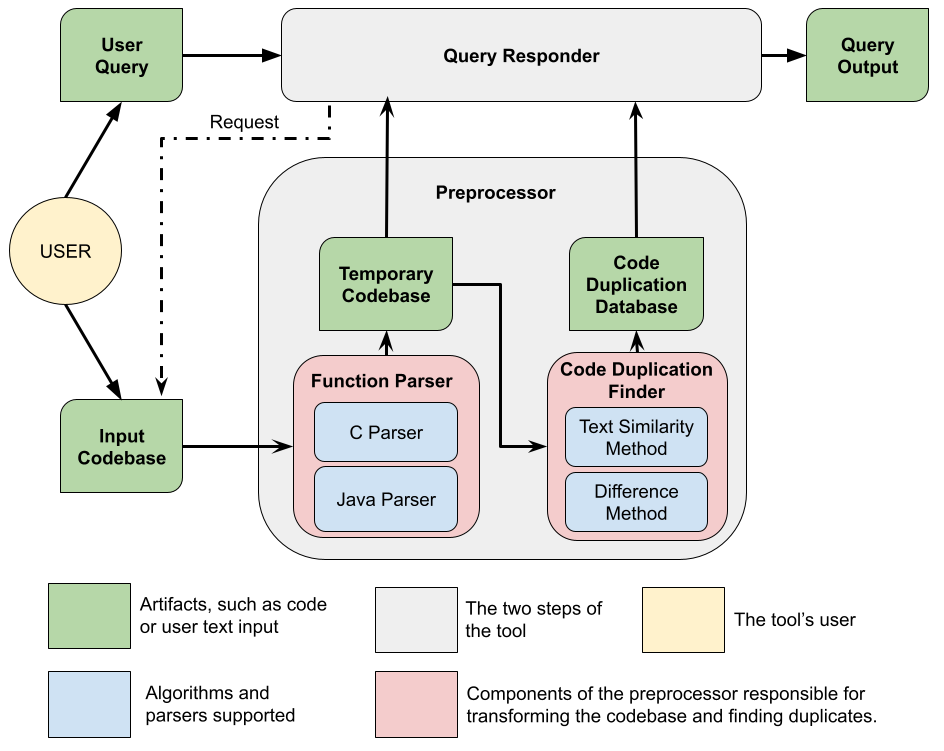
\includegraphics[width=3in]{diagrama_mestrado}
\caption{Architecture diagram demonstrating the relationship between the tool components}
\label{fig:diagram}
\end{figure}

The tool operates in two main parts: the \textbf{Preprocessor} and the \textbf{Query Responder}. 
The \textbf{Preprocessor} is responsible for performing heavy computations to find the code 
duplications across a codebase and produce artifacts to consult information related to the 
duplications in a structured form. The \textbf{Query Responder} consumes the artifacts produced 
by the Preprocessor to execute the tool functionalities as requested. This choice enables the 
tool to concentrate on the heavy and slow parts that can be executed only once per codebase, 
thus allowing a fast performance for multiple queries related to a single codebase.

The Preprocessor contains two main components, the Function Breaker and the Code Duplication Finder. 
The flow of how the Preprocessor works is as follow: Function Parser receives the codebase the user is interested in,
extracts the functions of the codebase along with metadata, and creates a new temporary codebase where the functions extracted become new code files. 
The Code Duplication Finder iterates over every pair of files in the Temporary Codebase, checks if they are code clones, and, 
if so, saves them in the Code Duplication Database, which is a text file that stores every code duplication as a triple 
\textbf{<function1,function2,similarity>}, where \textbf{function1} and \textbf{function2} are the functions that are duplicates 
of each other, and \textbf{similarity} is the metric given by the code duplication detection method utilized in the Code Duplication Finder.
Figure \ref{fig:diagram} illustrates the tool architecture.

The Query Responder consumes the Temporary Codebase and the Code Duplication Database to extract duplicated 
functions-related information per user request. If the user executes the Query Responder without executing the 
Preprocessor, the Query Responder calls the Preprocessor to create the required artifacts.

The Function Parser receives the input codebase and transforms it into the temporary
codebase. The Function Parser iterates through every source code file from the programming 
language it supports and uses a specific programming language function extractor
to extract every function in the file. For each function extracted, two new source code files
and a metadata file are created in the temporary codebase, represented by the pair <file
name, function name>, the source code file of the function, and the proper function.
The first new source code file contains the function’s body from the function it represents,
while the other new source code file contains the function’s signature. The metadata file
contains additional relevant information about the function, such as the function name,
the line where the function signature starts in the source code file, and the line where the
function’s body ends in the source code file. The programming languages supported at
the moment are C and Java, although Java has limited support.

The Code Duplication Finder iterates through every pair of source code files in the
temporary codebase, representing functions from the input codebase. For each pair of
files, we execute a code duplication detection method that computes a metric measuring
how similar the pair of files is, which we refer to as similarity. If the similarity is greater
than or equal to the minimum similarity threshold (a parameter provided by the user
during the Preprocessor), we store this pair of functions along with its similarity in the
Code Duplication Database. 
We implemented two methods for code duplication detection in the tool, which the user
can choose to use. The first method is based on text similarity, and the second is simpler
and based on the number of equal lines. The experiments and tests in this research were
done using the text similarity method.

\subsubsection{Code Duplication Methods Used}

For the text similarity method, we treat the source code files as text and apply the
TF-IDF vector embedding method implemented by the Gensim library \cite{gensim},
then compute cosine similarity as the similarity metric. This method was chosen for 
its claimed performance, programming language independence, and the fact that it does 
not require compilable code, which is expected in the
temporary codebase, as it does not contain complete code artifacts.

For the difference method, 
we implemented a method that considered the number of exactly equal lines between two functions.
For two functions \textit{function1} and \textit{function2}, we compute the similarity as the 
ratio of duplicated lines between the two functions by the total number of lines in both functions.
This code duplication method is considerably simpler and more explainable than the text similarity method, 
as the metric is the ratio of common lines between the two functions. To compute the number of equal lines, we use
the \textit{diff} command built-in in the Linux environment.

\subsection{Functionalities}

We propose three main functionalities for the user in the tool, called the Duplication
Explorer, Function Information, and Duplication Report. Each functionality accepts
specific parameters to perform its operations.

The Duplication Explorer is the primary functionality of our tool, designed to present
the user with pairs of duplicated functions identified by the tool. We implement optional
filters to facilitate more complex queries. Figure \ref{fig:explorer_ex} demonstrates an
example of this functionality in use.

\begin{figure}[!t]
\centering
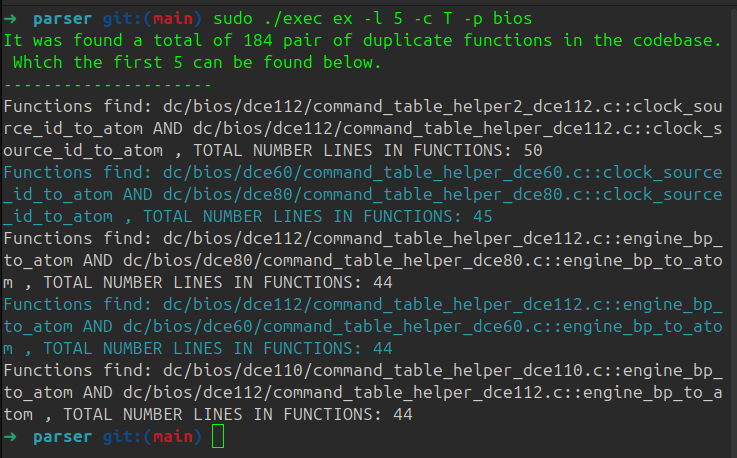
\includegraphics[width=3in]{explorer_example}
\caption{Example of the \textit{Duplication Explorer} functionality of the ArKanjo tool.}
\label{fig:explorer_ex}
\end{figure}

\begin{figure}[!t]
\centering
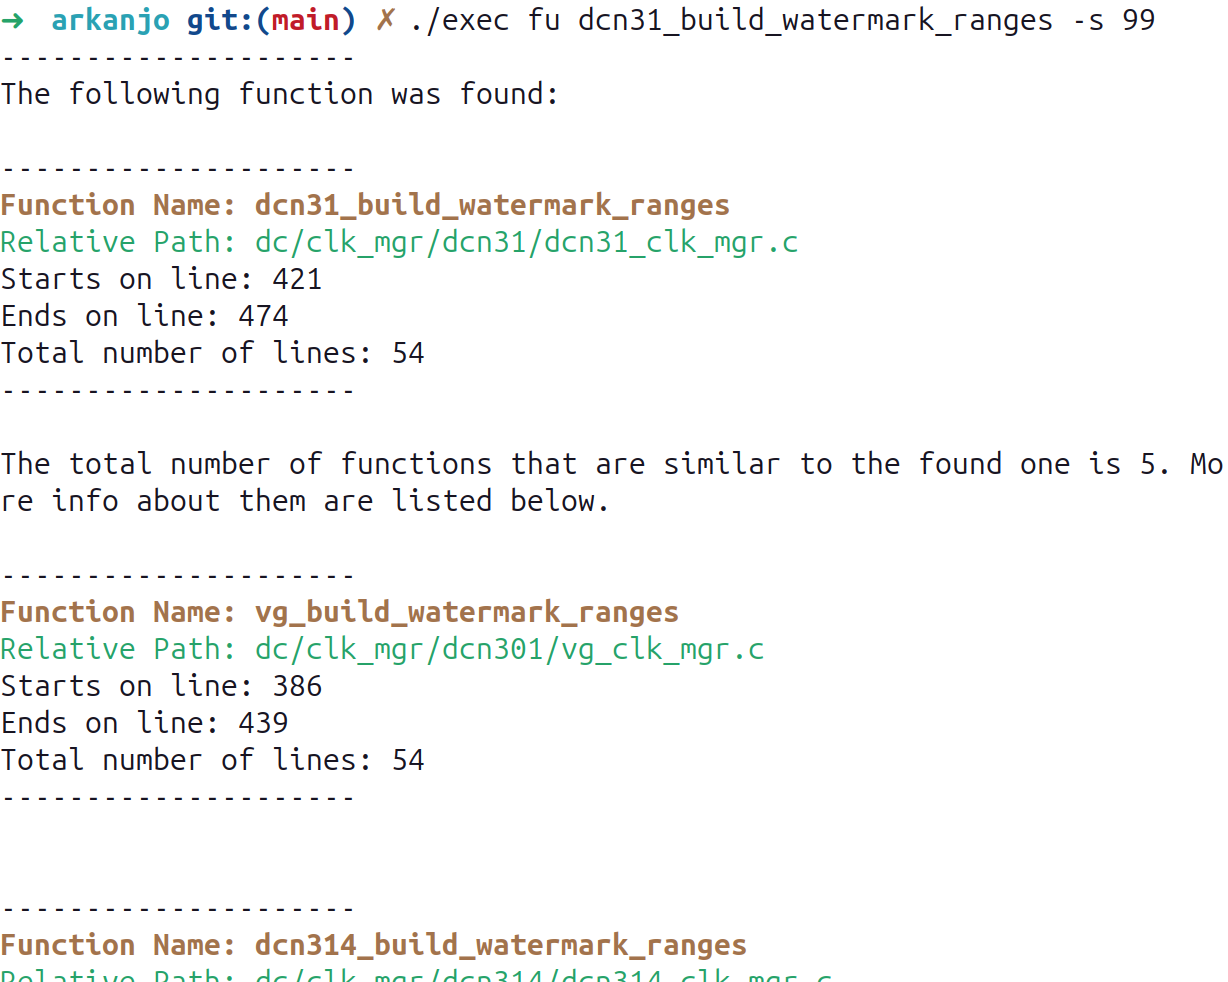
\includegraphics[width=3in]{function_example}
\caption{Example of the \textit{Function Information} functionality of the ArKanjo tool.}
\label{fig:function_ex}
\end{figure}

\begin{figure}[!t]
\centering
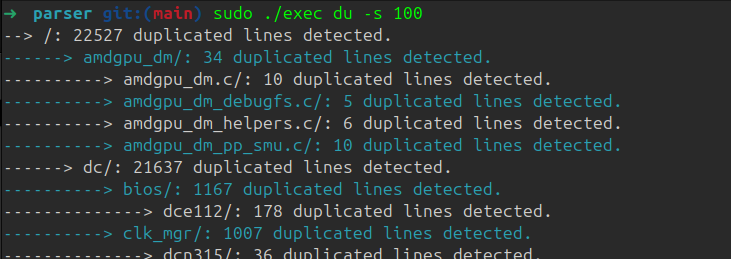
\includegraphics[width=3in]{relatory_example}
\caption{Example of the \textit{Duplication Report} functionality of the ArKanjo tool.}
\label{fig:relatory_ex}
\end{figure}


The Function Information functionality provides detailed information about a specific function. 
The functionality receives a target function from the user
and returns information such as the relative path, function name, and line numbers where
the function is defined. Additionally, it provides similar information for every function
that duplicates the given function. Figure \ref{fig:function_ex} demonstrates an
example of this functionality in use.

The Duplication Report functionality provides an overview of
duplicated code within the input codebase. This functionality calculates the number of
duplicated lines per folder in the codebase and presents the information to the user in
a readable format. Figure \ref{fig:relatory_ex} demonstrates an example of this functionality in use.

\section{Methods}

To validate the ArKanjo tool capabilities to find code duplications within the 
text similarity detection method used, we applied two independent
methods. The first method evaluates the proposed tool using an approach from the literature,
comparing it against the BigCloneBench dataset (Svajlenko et al., 2014). The second
method is an empirical analysis of a subset of functions within the AMD Display driver
that our tool identified as duplicates. 

To validate the tool against the BigCloneBench dataset \cite{bigclonebench}, we followed
the methodology presentedy by Liu et al. \cite{tailor}, we sampled 20,000 pairs from each clone
type, adding 20,000 non-duplicate pairs as negative samples. We applied the same sampling
approach to our tool to ensure a fair evaluation.
Unlike state-of-art methods, our tool does not distinguish between clone types and
identifies duplications at the function level rather than the file level, which is typical in
state-of-the-art tools. Therefore, we adapted the metric calculation method for evaluation
purposes. Specifically, we considered every pair of functions with a similarity metric
equal to or greater than a threshold X as duplicates and marked the corresponding file
pairs. A correctly identified duplication pair counts as accurate for its clone type, while
an incorrectly inferred pair is considered incorrect across all clone types.
To understand the impact of varying the similarity threshold, we evaluated our tool using
different threshold values: 30\%, 40\%, 50\%, 60\%, 70\%, 80\%, 90\%, and 100\%. We then analyzed
and discussed the results.

For the empirical analysis, we randomly sampled function pairs identified by the tool as
duplicates. For each similarity threshold X (30\%, 40\%, 50\%, 60\%, 70\%, 80\%, 90\%, and 100\%) 
we randomly selected ten function pairs with a similarity close to X, allowing for a 1\%
deviation.

To assess if the duplications found by the ArKanjo tool were actionable, the research conducted 
a multi-part ethnographic study. In this study, the author and 12 student groups from the
Free Software Development course at University of São Paulo acted as new contributors 
to the Linux kernel. 
They used the tool to identify duplications within the Industrial I/O (IIO) subsytem and AMD Display 
driver subsystems, refactored the code to address the issues, and submitted their proposed 
fixes as patches to the community maintainers. Throughout this process, the students documented 
their refactoring approaches and their experiences interacting with the kernel community.

\section{Results}

\subsection{Tool Evaluation}

\begin{table}[!t]

\centering

\renewcommand{\arraystretch}{1.3}
\begin{tabular}{ | m{13mm} | c | c | c | c | m{6mm} | m{6mm} | }

\hline

\textbf{Similarity Threshould} & \textbf{T1} & \textbf{T2} & ST3 & MT3
& WT3/ T4 & \textbf{False} \\ \hline

100\% & 100\% & 5\% & 6\% & 0\% & 0\% & 100\% \\ \hline
90\% & 100\% & 85\% & 26\% & 0\% & 0\% & 100\% \\ \hline
80\% & 100\% & 87\% & 37\% & 1\% & 0\% & 100\% \\ \hline
70\% & 100\% & 88\% & 44\% & 2\% & 0\% & 100\% \\ \hline
60\% & 100\% & 89\% & 49\% & 4\% & 0\% & 100\% \\ \hline
50\% & 100\% & 90\% & 64\% & 6\% & 0\% & 100\% \\ \hline
40\% & 100\% & 90\% & 68\% & 9\% & 0\% & 100\% \\ \hline
30\% & 100\% & 98\% & 74\% & 13\% & 0\% & 100\% \\ \hline

\hline
\end{tabular}
\caption{Recall of the ArKanjo tool in the BigCloneBench dataset varying minimum similarity threshould.}
\label{tab:bigclone}
\end{table}

\begin{table}[!t]

\centering

\begin{tabular}{ | m{15mm} | c | c | c | c | m{6mm} | m{10mm} | }

\hline

\textbf{Similarity range} & \textbf{T1} & \textbf{T2} & T3 & T4
& \textbf{False} & \textbf{Success Percentage} \\ \hline
99\% - 100\% & 9 & 0 & 0 & 1 & 0 & \textbf{100\%} \\ \hline
89\% - 91\% & 0 & 8 & 0 & 1 & 1 & \textbf{90\%} \\ \hline
79\% - 81\% & 0 & 3 & 2 & 3 & 2 & \textbf{80\%} \\ \hline
69\% - 71\% & 0 & 3 & 1 & 1 & 5 & \textbf{50\%} \\ \hline
59\% - 61\% & 0 & 0 & 0 & 2 & 8 & \textbf{20\%} \\ \hline
49\% - 51\% & 0 & 0 & 0 & 0 & 10 & \textbf{0\%} \\ \hline
39\% - 41\% & 0 & 0 & 0 & 0 & 10 & \textbf{0\%} \\ \hline
29\% - 31\% & 0 & 0 & 0 & 0 & 10 & \textbf{0\%} \\ \hline

\hline

\end{tabular}
\caption{Results of the ArKanjo tool in the empirical analyses in the AMD Display driver}
\label{tab:emp}

\end{table}

Table \ref{tab:bigclone} shows the results obtained by our tool on the BigCLoneBench dataset
and table \ref{tab:emp} shows the results obtained in the empricial analysis.
The BigCloneBench results and our empirical methods indicate that our tool performs
well in detecting Type-1 and Type-2 code clone duplications and can thus reveal propagated 
issues like copied buggy logic, but it struggles with more
complex types. A similarity threshold between 80\% and 100\% yields favorable results
in both methods. 

However, there is a discrepancy in the detection of non-duplication pairs between
the two methods. In the BigCloneBench evaluation, we found no false positives (negative
samples inferred as duplications), while the empirical analysis revealed a higher percentage
of false positives. We propose two potential explanations for this discrepancy.

The first reason may be the limitations and known issues with BigCloneBench, as
highlighted by Krinke and Ragkhitwetsagul \cite{bigfail}. The
second reason could relate to the nature of the AMD Display driver, where each code artifact
shares semantic meaning. In contrast, BigCloneBench comprises self-contained code
artifacts without shared semantics. Given that our tool relies on a text-based code clone
detection approach, it may naturally perform worse on the AMD Display driver than on the
BigCloneBench dataset.

\subsection{Ethnographic Study}

Using the ArKanjo tool, the author and 12 student groups identified and refactored duplicated 
code in the AMD Display driver and the Industrial I/O (IIO) subsystems, submitting their work 
as patches to the community maintainers. This effort resulted in 13 total patch submissions: 
one from the author to the AMD Display driver and 12 from the student groups, with 11 targeting 
the IIO subsystem and one for the AMD Display driver. The author's patch, which removed over 
500 lines of duplicated code, was successfully accepted and merged into the kernel after a 
lengthy review process.

The student efforts showed that newcomers could use the tool to make effective contributions. 
Of the 12 student patches, five were accepted, four were refused, and three required follow-up 
fixes based on maintainer feedback. To remove the duplicated code, seven student groups used the 
Parameterize Method and two used the Extract Method \cite{refactorbook}, which are simple refactoring methods. 
This result corroborates that ArKanjo finds actionable duplications and that newcomers can 
successfully contribute patches to the kernel.

While this research included a successfully merged patch by the author and students,
a notable portion of student efforts encountered
significant hurdles. These difficulties often stemmed from maintainer feedback where
proposed changes, though reducing duplication, were rejected or required substantial
rework due to concerns about code readability, added abstraction, or the specific context
of the code. Technical complexities, such as C macros in configuration files, and lengthy
patch review times also contributed to the challenges. 
This highlights that while ArKanjo effectively identifies duplications, a successful 
contribution involves a trade-off between code deduplication and other factors like the 
specific code's context and maintainer priorities.

\section{Conclusion}

In conclusion, this paper presented ArKanjo, a novel tool designed to effectively detect 
and facilitate the refactoring of function-level code duplication within the Linux kernel. 
Evaluations demonstrated that ArKanjo is highly effective at identifying Type-1 and Type-2 
clones, which are often indicative of propagated issues like copied buggy logic. The practical 
value of the tool was confirmed through an ethnographic study where the author and student 
groups used ArKanjo to identify actionable duplications. This effort led to 13 patch 
submissions, including one from the author that removed over 500 lines of code and was merged 
into the kernel, alongside three successful student contributions. While some refactoring 
efforts were declined due to maintainer priorities, ArKanjo successfully lowers the barrier 
for new contributors to make meaningful improvements. The tool provides immediate value for 
kernel maintenance and serves as a model for clone detection in other large-scale projects.


% An example of a floating figure using the graphicx package.
% Note that \label must occur AFTER (or within) \caption.
% For figures, \caption should occur after the \includegraphics.
% Note that IEEEtran v1.7 and later has special internal code that
% is designed to preserve the operation of \label within \caption
% even when the captionsoff option is in effect. However, because
% of issues like this, it may be the safest practice to put all your
% \label just after \caption rather than within \caption{}.
%
% Reminder: the "draftcls" or "draftclsnofoot", not "draft", class
% option should be used if it is desired that the figures are to be
% displayed while in draft mode.
%
%\begin{figure}[!t]
%\centering
%\includegraphics[width=2.5in]{myfigure}
% where an .eps filename suffix will be assumed under latex, 
% and a .pdf suffix will be assumed for pdflatex; or what has been declared
% via \DeclareGraphicsExtensions.
%\caption{Simulation results for the network.}
%\label{fig_sim}
%\end{figure}

% Note that the IEEE typically puts floats only at the top, even when this
% results in a large percentage of a column being occupied by floats.


% An example of a double column floating figure using two subfigures.
% (The subfig.sty package must be loaded for this to work.)
% The subfigure \label commands are set within each subfloat command,
% and the \label for the overall figure must come after \caption.
% \hfil is used as a separator to get equal spacing.
% Watch out that the combined width of all the subfigures on a 
% line do not exceed the text width or a line break will occur.
%
%\begin{figure*}[!t]
%\centering
%\subfloat[Case I]{\includegraphics[width=2.5in]{box}%
%\label{fig_first_case}}
%\hfil
%\subfloat[Case II]{\includegraphics[width=2.5in]{box}%
%\label{fig_second_case}}
%\caption{Simulation results for the network.}
%\label{fig_sim}
%\end{figure*}
%
% Note that often IEEE papers with subfigures do not employ subfigure
% captions (using the optional argument to \subfloat[]), but instead will
% reference/describe all of them (a), (b), etc., within the main caption.
% Be aware that for subfig.sty to generate the (a), (b), etc., subfigure
% labels, the optional argument to \subfloat must be present. If a
% subcaption is not desired, just leave its contents blank,
% e.g., \subfloat[].


% An example of a floating table. Note that, for IEEE style tables, the
% \caption command should come BEFORE the table and, given that table
% captions serve much like titles, are usually capitalized except for words
% such as a, an, and, as, at, but, by, for, in, nor, of, on, or, the, to
% and up, which are usually not capitalized unless they are the first or
% last word of the caption. Table text will default to \footnotesize as
% the IEEE normally uses this smaller font for tables.
% The \label must come after \caption as always.
%
%\begin{table}[!t]
%% increase table row spacing, adjust to taste
%\renewcommand{\arraystretch}{1.3}
% if using array.sty, it might be a good idea to tweak the value of
% \extrarowheight as needed to properly center the text within the cells
%\caption{An Example of a Table}
%\label{table_example}
%\centering
%% Some packages, such as MDW tools, offer better commands for making tables
%% than the plain LaTeX2e tabular which is used here.
%\begin{tabular}{|c||c|}
%\hline
%One & Two\\
%\hline
%Three & Four\\
%\hline
%\end{tabular}
%\end{table}


% Note that the IEEE does not put floats in the very first column
% - or typically anywhere on the first page for that matter. Also,
% in-text middle ("here") positioning is typically not used, but it
% is allowed and encouraged for Computer Society conferences (but
% not Computer Society journals). Most IEEE journals/conferences use
% top floats exclusively. 
% Note that, LaTeX2e, unlike IEEE journals/conferences, places
% footnotes above bottom floats. This can be corrected via the
% \fnbelowfloat command of the stfloats package.




% conference papers do not normally have an appendix


% use section* for acknowledgment

% trigger a \newpage just before the given reference
% number - used to balance the columns on the last page
% adjust value as needed - may need to be readjusted if
% the document is modified later
%\IEEEtriggeratref{8}
% The "triggered" command can be changed if desired:
%\IEEEtriggercmd{\enlargethispage{-5in}}

% references section

% can use a bibliography generated by BibTeX as a .bbl file
% BibTeX documentation can be easily obtained at:
% http://mirror.ctan.org/biblio/bibtex/contrib/doc/
% The IEEEtran BibTeX style support page is at:
% http://www.michaelshell.org/tex/ieeetran/bibtex/
\bibliographystyle{IEEEtran}
% argument is your BibTeX string definitions and bibliography database(s)
\bibliography{IEEEabrv,referencias}
%
% <OR> manually copy in the resultant .bbl file
% set second argument of \begin to the number of references
% (used to reserve space for the reference number labels box)
% \begin{thebibliography}{1}
%  
%  \bibitem{IEEEhowto:kopka}
%  H.~Kopka and P.~W. Daly, \emph{A Guide to \LaTeX}, 3rd~ed.\hskip 1em plus
%    0.5em minus 0.4em\relax Harlow, England: Addison-Wesley, 1999.
%  
% \end{thebibliography}




% that's all folks
\end{document}


